\documentclass{article}
\usepackage{amsmath,booktabs}
\usepackage{tikz}
\usepackage[a4paper,margin=2.5cm]{geometry}
\title{Exercise: FAST Interaction Detection with Prefix Sums}
\date{}
\begin{document}
\author{}
\maketitle

\section*{Exercise}
The table lists \(n=9\) samples with two numerical features and a target:

\begin{center}
\begin{tabular}{ccccc}
\toprule
Idx & $x_1$ & $x_2$ & $y$ \\ \midrule
0 & 1.07 & 1.11 &  2 \\
1 & 1.86 & 1.05 &  3\\
2 & 3.18 & 1.07 &  4 \\
3 & 0.93 & 2.16 &  5 \\
4 & 2.12 & 2.08 &  6 \\
5 & 2.85 & 2.14 &  7 \\
6 & 1.18 & 3.06 &  8 \\
7 & 2.03 & 2.92 &  9 \\
8 & 3.09 & 3.17 & 10 \\ \bottomrule
\end{tabular}

\end{center}

\bigskip
\textbf{Tasks}
\begin{enumerate}
\item Discretize each feature into three equal-width bins  
      \([0,1.5)\!\to\!0,\;[1.5,2.5)\!\to\!1,\;[2.5,3.5)\!\to\!2\).

\item Build two \(3\times3\) matrices
      \[
        S(i,j)=\!\!\sum_{(x_1^b,x_2^b)=(i,j)} \! y,
        \qquad
        N(i,j)=\!\!\sum_{(x_1^b,x_2^b)=(i,j)} \! 1 .
      \]

\item Form 2-D prefix sums
      \(S^{\mathrm{pref}},N^{\mathrm{pref}}\).

\item Via inclusion–exclusion obtain totals for the rectangle  
      \(x_1^b\!\in\!\{1,2\},\,x_2^b\!\in\!\{1,2\}\):  
      \(S_r,\;N_r\).

\item Compute the mean in this region:
      \(\hat y_r = S_r/N_r\).

\item Let \(S_n=\sum_{i=1}^n y^{(i)},\;N_n=n\).  
      Show that the \emph{RSS reduction}
      \[
        \Delta\text{RSS}
          = \frac{S_r^{\,2}}{N_r}
            +\frac{(S_n-S_r)^{2}}{N_n-N_r}
            -\frac{S_n^{\,2}}{N_n}
      \]
      needs only first-order sums (no \(y^2\)).
\end{enumerate}

\section*{Solution}

\subsection*{1.~Binning the data}

\begin{center}
% \begin{tabular}{ccccc}
% \toprule
% Idx & $x_1$ & $x_2$ & $y$ & $(x_1^b,x_2^b)$\\ \midrule
% 0 &1&1&2 &(0,0)\\
% 1 &2&1&3 &(1,0)\\
% 2 &3&1&4 &(2,0)\\
% 3 &1&2&5 &(0,1)\\
% 4 &2&2&6 &(1,1)\\
% 5 &3&2&7 &(2,1)\\
% 6 &1&3&8 &(0,2)\\
% 7 &2&3&9 &(1,2)\\
% 8 &3&3&10&(2,2)\\ \bottomrule
% \end{tabular}
\begin{tabular}{ccccc}
\toprule
Idx & $x_1$ & $x_2$ & $y$ & $(x_1^b,x_2^b)$\\ \midrule
0 & 1.07 & 1.11 &  2 & (0,0)\\
1 & 1.86 & 1.05 &  3 & (1,0)\\
2 & 3.18 & 1.07 &  4 & (2,0)\\
3 & 0.93 & 2.16 &  5 & (0,1)\\
4 & 2.12 & 2.08 &  6 & (1,1)\\
5 & 2.85 & 2.14 &  7 & (2,1)\\
6 & 1.18 & 3.06 &  8 & (0,2)\\
7 & 2.03 & 2.92 &  9 & (1,2)\\
8 & 3.09 & 3.17 & 10 & (2,2)\\ \bottomrule
\end{tabular}

\end{center}

\subsection*{2.~Aggregate matrices \(S\) and \(N\)}
\[
  S=\begin{bmatrix}
        2 & 5 & 8\\
        3 & 6 & 9\\
        4 & 7 & 10
     \end{bmatrix},
\qquad
  N=\begin{bmatrix}
        1&1&1\\
        1&1&1\\
        1&1&1
     \end{bmatrix}
\]

\subsection*{3.~2-D prefix sums}
\[
  S^{\text{pref}}=\begin{bmatrix}
      2 & 7 & 15\\
      5 & 16& 33\\
      9 & 27& 54
  \end{bmatrix},
\qquad
  N^{\text{pref}}=\begin{bmatrix}
      1 & 2 & 3\\
      2 & 4 & 6\\
      3 & 6 & 9
  \end{bmatrix}
\]

\subsection*{4.~Rectangle \((1{:}2,1{:}2)\)}

% ------------------------------------------------------------
% --- Inclusion–Exclusion on a 2-D Prefix-Sum Grid -----------
% ------------------------------------------------------------
%\subsection*{4.~General inclusion--exclusion for any rectangle}

Let the binned grid have indices \(0,\dots,B-1\) on each axis and define an
axis-aligned rectangle
\[
  R=[i_{\min}\!:\!i_{\max}]\;\times\;[j_{\min}\!:\!j_{\max}],
  \qquad
  0\le i_{\min}\le i_{\max}<B,\;
  0\le j_{\min}\le j_{\max}<B .
\]

With 2-D prefix sums
\[
  S^{\mathrm{pref}}(i,j)=\!\!\!\sum_{u\le i,\;v\le j}\!S(u,v),
  \qquad
  N^{\mathrm{pref}}(i,j)=\!\!\!\sum_{u\le i,\;v\le j}\!N(u,v),
\]
the totals in \(R\) are obtained via inclusion–exclusion:
\begin{equation}
\boxed{
\begin{aligned}
  S_R &= S^{\mathrm{pref}}_{i_{\max},j_{\max}}
         -S^{\mathrm{pref}}_{i_{\min}-1,j_{\max}}
         -S^{\mathrm{pref}}_{i_{\max},\,j_{\min}-1}
         +S^{\mathrm{pref}}_{i_{\min}-1,\,j_{\min}-1},\\[4pt]
  N_R &= N^{\mathrm{pref}}_{i_{\max},j_{\max}}
         -N^{\mathrm{pref}}_{i_{\min}-1,j_{\max}}
         -N^{\mathrm{pref}}_{i_{\max},\,j_{\min}-1}
         +N^{\mathrm{pref}}_{i_{\min}-1,\,j_{\min}-1}.
\end{aligned}}
\label{eq:2D-inc-exc}
\end{equation}
(All terms with index \(-1\) are interpreted as zero.)


% ------------------------------------------------------------
% Illustration: 2-D prefix sums and inclusion–exclusion
% ------------------------------------------------------------
\begin{figure}[h]
\centering
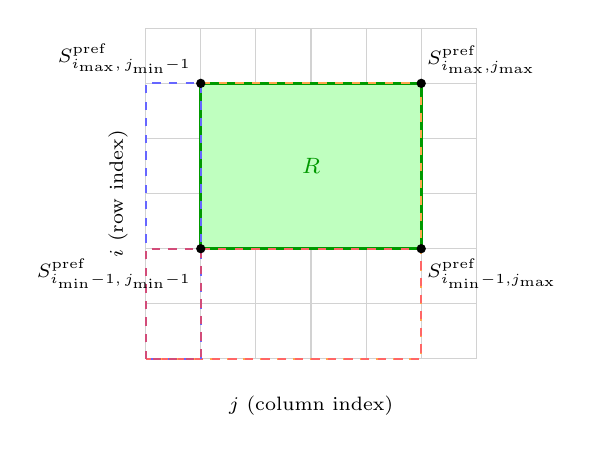
\begin{tikzpicture}[scale=0.7,>=latex,
        every node/.style={font=\scriptsize}]
  % ------- parameters (example values for visualisation) --------
  \def\B{6}          % grid size  B×B
  \def\imin{2}\def\imax{4}
  \def\jmin{1}\def\jmax{4}

  % ------- background grid --------------------------------------
  \foreach \i in {0,...,\B}{
    \draw[gray!35] (0,\i) -- (\B,\i);
    \draw[gray!35] (\i,0) -- (\i,\B);
  }

  % ------- target rectangle R -----------------------------------
  \fill[green!25]   (\jmin,\imin) rectangle (\jmax+1,\imax+1);
  \draw[green!60!black,very thick]
        (\jmin,\imin) rectangle (\jmax+1,\imax+1)
        node[midway,font=\footnotesize] {$R$};

  % ------- four prefix rectangles used in Eq. (1) ---------------
  % + S_pref(i_max,j_max)
  \draw[orange!70,thick,dashed] (0,0) rectangle (\jmax+1,\imax+1);
  % - S_pref(i_min-1,j_max)
  \draw[red!60,thick,dashed]    (0,0) rectangle (\jmax+1,\imin);
  % - S_pref(i_max,j_min-1)
  \draw[blue!60,thick,dashed]   (0,0) rectangle (\jmin,\imax+1);
  % + S_pref(i_min-1,j_min-1)
  \draw[purple!70,thick,dashed] (0,0) rectangle (\jmin,\imin);

  % ------- markers at the four prefix–sum coordinates -----------
  \fill (\jmax+1,\imax+1) circle (2.4pt)
        node[above right] {$\!S^{\text{pref}}_{i_{\max},j_{\max}}$};
  \fill (\jmax+1,\imin)   circle (2.4pt)
        node[below right] {$\!S^{\text{pref}}_{i_{\min}-1,j_{\max}}$};
  \fill (\jmin,\imax+1)   circle (2.4pt)
        node[above left]  {$S^{\text{pref}}_{i_{\max},\,j_{\min}-1}$};
  \fill (\jmin,\imin)     circle (2.4pt)
        node[below left]  {$S^{\text{pref}}_{i_{\min}-1,\,j_{\min}-1}$};

  % ------- axes labels ------------------------------------------
  \node[below] at (\B/2,-0.5) {$j$ (column index)};
  \node[rotate=90] at (-0.5,\B/2) {$i$ (row index)};
\end{tikzpicture}
\caption{Inclusion--exclusion on a 2-D prefix grid.
The green area is the query rectangle \(R\).
Dashed rectangles show the four prefix sums employed in
Eq.~\eqref{eq:2D-inc-exc}:
orange \((+)\), red and blue \((-)\), purple \((+)\).}
\label{fig:2D-prefix-inc-exc}
\end{figure}

\medskip
Using the same four look-ups one can obtain the subtotals of the
\emph{other three} regions that partition the orange prefix rectangle:

\[
\begin{aligned}
S_{\text{top}} &=
  S^{\text{pref}}_{\,i_{\min}-1,j_{\max}}
  -S^{\text{pref}}_{\,i_{\min}-1,j_{\min}-1}, \\[4pt]
S_{\text{left}} &=
  S^{\text{pref}}_{\,i_{\max},j_{\min}-1}
  -S^{\text{pref}}_{\,i_{\min}-1,j_{\min}-1}, \\[4pt]
S_{\text{topleft}} &=
  S^{\text{pref}}_{\,i_{\min}-1,j_{\min}-1}\;.
\end{aligned}
\]
(Replace \(S^{\text{pref}}\) by \(N^{\text{pref}}\) to get the
corresponding counts.)

\bigskip
\noindent
\textbf{RSS drop using only first-order sums.}  
Let \(S_n=\sum_{i=1}^{n}y^{(i)}\) and \(N_n=n\).  Define
\(S_C=S_n-S_R\) and \(N_C=N_n-N_R\).  Then the reduction in residual
sum of squares when isolating rectangle \(R\) is
\begin{equation}
\boxed{\displaystyle
  \Delta\text{RSS}(R)=
      \frac{S_R^{2}}{N_R}
     +\frac{S_C^{2}}{N_C}
     -\frac{S_n^{2}}{N_n}},
\label{eq:rss-drop}
\end{equation}
which involves \emph{only} the first-order target sums \(S_\bullet\) and
counts \(N_\bullet\); all \(\sum y^{2}\) terms cancel.  This identity is
the core of the FAST interaction-search algorithm and the 1-D
prefix-sum split optimisation presented in the lecture.

Using inclusion–exclusion:
\[
\begin{aligned}
S_r &= S^{\text{pref}}_{2,2}-S^{\text{pref}}_{0,2}
      -S^{\text{pref}}_{2,0}+S^{\text{pref}}_{0,0}=54-15-9+2=32,\\
N_r &= N^{\text{pref}}_{2,2}-N^{\text{pref}}_{0,2}
      -N^{\text{pref}}_{2,0}+N^{\text{pref}}_{0,0}=9-3-3+1=4.
\end{aligned}
\]

\subsection*{5.~Mean prediction}
\[
  \hat y_r = \frac{S_r}{N_r}= \frac{32}{4}=8 .
\]

\subsection*{6.~RSS reduction with first-order sums only}
Total sums: \(S_n=54,\;N_n=9\).  
Complement: \(S_c=S_n-S_r=22,\;N_c=N_n-N_r=5\).

\[
\boxed{\displaystyle
  \Delta\text{RSS}
    =\frac{S_r^{2}}{N_r}
     +\frac{S_c^{2}}{N_c}
     -\frac{S_n^{2}}{N_n}
    =\frac{32^{2}}{4}+\frac{22^{2}}{5}-\frac{54^{2}}{9}
    =28.8 } 
\]

\medskip
\noindent
\emph{Observation:} The formula contains only the sums \(S\) and counts \(N\); all
\(\sum y^{2}\) terms cancel.  This is exactly the trick exploited by FAST
and the prefix-sum split algorithm in the lecture.

\end{document}


% \documentclass{article}
% \usepackage{amsmath, booktabs}
% \usepackage[a4paper,margin=2.5cm]{geometry}
% \usepackage{tikz}
% \title{Exercise: FAST Interaction Detection with Prefix Sums}
% \date{}
% \begin{document}
% \maketitle

% \section*{Exercise}
% You are given the following dataset of 9 samples, each with two numeric features $x_1$, $x_2$ and a numeric target $y$:

% \begin{center}
% \begin{tabular}{cccc}
% \toprule
% Index & $x_1$ & $x_2$ & $y$ \\
% \midrule
% 0 & 1 & 1 & 2 \\
% 1 & 2 & 1 & 3 \\
% 2 & 3 & 1 & 4 \\
% 3 & 1 & 2 & 5 \\
% 4 & 2 & 2 & 6 \\
% 5 & 3 & 2 & 7 \\
% 6 & 1 & 3 & 8 \\
% 7 & 2 & 3 & 9 \\
% 8 & 3 & 3 & 10 \\
% \bottomrule
% \end{tabular}
% \end{center}

% \bigskip

% \textbf{Tasks:}
% \begin{enumerate}
%     \item Discretize $x_1$ and $x_2$ into 3 equal-width bins: $[0,1.5)$, $[1.5,2.5)$, $[2.5,3.5)$, mapping to bin indices 0, 1, and 2.

%     \item Construct 3 matrices $T(i,j)$, $Q(i,j)$, and $N(i,j)$ of size $3 \times 3$ where:
%     \begin{itemize}
%         \item $T(i,j)$ = sum of $y$ in bin $(i,j)$
%         \item $Q(i,j)$ = sum of $y^2$ in bin $(i,j)$
%         \item $N(i,j)$ = number of observations in bin $(i,j)$
%     \end{itemize}

%     \item Compute the prefix sums for each of $T$, $Q$, and $N$ using 2D cumulative summation.

%     \item Using inclusion--exclusion, compute the total $T_r$, $Q_r$, and $N_r$ in the bottom-right $2 \times 2$ region: $x_1 \in \{1,2\}$ and $x_2 \in \{1,2\}$.

%     \item Compute the mean prediction $\hat{y}_r = T_r / N_r$.

%     \item Compute the Residual Sum of Squares (RSS) as:
%     \[
%     \text{RSS} = Q_r - \frac{T_r^2}{N_r}
%     \]
% \end{enumerate}

% \section*{Solution}

% \subsection*{Binned Data}
% Bin indices $(x_1, x_2) \to (x_1^b, x_2^b)$:

% \begin{center}
% \begin{tabular}{ccccc}
% \toprule
% Index & $x_1$ & $x_2$ & $y$ & $(x_1^b, x_2^b)$ \\
% \midrule
% 0 & 1 & 1 & 2 & (0,0) \\
% 1 & 2 & 1 & 3 & (1,0) \\
% 2 & 3 & 1 & 4 & (2,0) \\
% 3 & 1 & 2 & 5 & (0,1) \\
% 4 & 2 & 2 & 6 & (1,1) \\
% 5 & 3 & 2 & 7 & (2,1) \\
% 6 & 1 & 3 & 8 & (0,2) \\
% 7 & 2 & 3 & 9 & (1,2) \\
% 8 & 3 & 3 & 10 & (2,2) \\
% \bottomrule
% \end{tabular}
% \end{center}

% \subsection*{Aggregate Matrices}

% \begin{itemize}
%     \item $T$ (sum of $y$):
%     \[ T = \begin{bmatrix} 2 & 5 & 8 \\ 3 & 6 & 9 \\ 4 & 7 & 10 \end{bmatrix} \]

%     \item $Q$ (sum of $y^2$):
%     \[ Q = \begin{bmatrix} 4 & 25 & 64 \\ 9 & 36 & 81 \\ 16 & 49 & 100 \end{bmatrix} \]

%     \item $N$ (counts):
%     \[ N = \begin{bmatrix} 1 & 1 & 1 \\ 1 & 1 & 1 \\ 1 & 1 & 1 \end{bmatrix} \]
% \end{itemize}

% \subsection*{Prefix Sums}
% Apply cumulative summation along both axes:

% \begin{itemize}
%     \item $T^{\text{prefix}} = \begin{bmatrix} 2 & 7 & 15 \\ 5 & 16 & 33 \\ 9 & 27 & 54 \end{bmatrix}$
%     \item $Q^{\text{prefix}} = \begin{bmatrix} 4 & 29 & 93 \\ 13 & 74 & 219 \\ 29 & 139 & 319 \end{bmatrix}$
%     \item $N^{\text{prefix}} = \begin{bmatrix} 1 & 2 & 3 \\ 2 & 4 & 6 \\ 3 & 6 & 9 \end{bmatrix}$
% \end{itemize}

% \subsection*{Region: Bottom-right $2 \times 2$}
% Bin range: $x_1^b \in \{1,2\},\ x_2^b \in \{1,2\}$, i.e., region from $(1,1)$ to $(2,2)$.
% Use inclusion--exclusion:
% \begin{align*}
% T_r &= T_{2,2} - T_{0,2} - T_{2,0} + T_{0,0} = 54 - 15 - 9 + 2 = 32 \\
% Q_r &= Q_{2,2} - Q_{0,2} - Q_{2,0} + Q_{0,0} = 319 - 93 - 29 + 4 = 201 \\
% N_r &= N_{2,2} - N_{0,2} - N_{2,0} + N_{0,0} = 9 - 3 - 3 + 1 = 4
% \end{align*}

% \subsection*{RSS Computation}
% \begin{align*}
% \hat{y}_r &= \frac{T_r}{N_r} = \frac{32}{4} = 8 \\
% \text{RSS} &= Q_r - \frac{T_r^2}{N_r} = 201 - \frac{32^2}{4} = 201 - 256 = \boxed{10}
% \end{align*}

% \end{document}
